\documentclass[aspectratio=169]{beamer}


\mode<presentation>
{
	\usetheme{Singapore}      % or try Darmstadt, Madrid, Warsaw, ...
	\usecolortheme{whale} % or try albatross, beaver, crane, ...
	\usefonttheme{default}  % or try serif, structurebold, ...
	\setbeamertemplate{navigation symbols}{}
	\setbeamertemplate{caption}[numbered]
}

%enumerate continuing numbering
\setbeamercovered{highly dynamic}

\newcounter{saveenumi}
\newcommand{\seti}{\setcounter{saveenumi}{\value{enumi}}}
\newcommand{\conti}{\setcounter{enumi}{\value{saveenumi}}}
%

\usepackage[portuguese]{babel}
\usepackage[utf8x]{inputenc}
\usepackage[T1]{fontenc}
\usepackage{natbib}
\usepackage{hyperref}
\usepackage{enumerate}
%\usepackage{biblatex}

%numbering
\addtobeamertemplate{navigation symbols}{}{%
	\usebeamerfont{footline}%
	\usebeamercolor[fg]{footline}%
	\hspace{1em}%
	\insertframenumber/\inserttotalframenumber
}

\title[Your Short Title]{Aprimoramentos em modelagem geológica implícita com funções distância assinaladas}
\subtitle{Proposta de tese para o exame de qualificação}
\author{Me. Roberto Mentzingen Rolo \\ \small{Orientador: Prof. Dr. João Felipe Coimbra Leite Costa, PhD}}
\institute{Universidade Federal do Rio Grande do Sul \\ Escola de Engenharia \\ Programa de Pós-Graduação em Engenharia de Minas, Metalúrgica e de Materiais}
\date{17 de junho de 2019}

\begin{document}
	
\section{Apresentação}
	
\begin{frame}
	\titlepage
\end{frame}

%sumário
\begin{frame}{Estrutura}
\begin{scriptsize}
	\tableofcontents
\end{scriptsize}
\end{frame}

\section{Introdução}

\begin{frame}{Introdução}

Construir modelos numéricos de longo, médio e curto prazo para avaliação de recursos/reservas e planejamento de mina exige quatro grandes atividades:

\begin{enumerate}
\item Coleta e gerenciamento de dados;
\item Interpretação e modelagem geológica;
\item Atribuição de teores;
\item Avaliação e gerenciamento da incerteza geológica e de teores.
\end{enumerate}

\end{frame}

\subsection{Interpretação e modelagem geológica}

\begin{frame}{Interpretação e modelagem geológica}

\begin{enumerate}
	\item Identificar diferentes domínios;
	\item Definir os limites de cada função aleatória estacionária.
\end{enumerate}

\begin{figure}[H]
	\begin{center}
		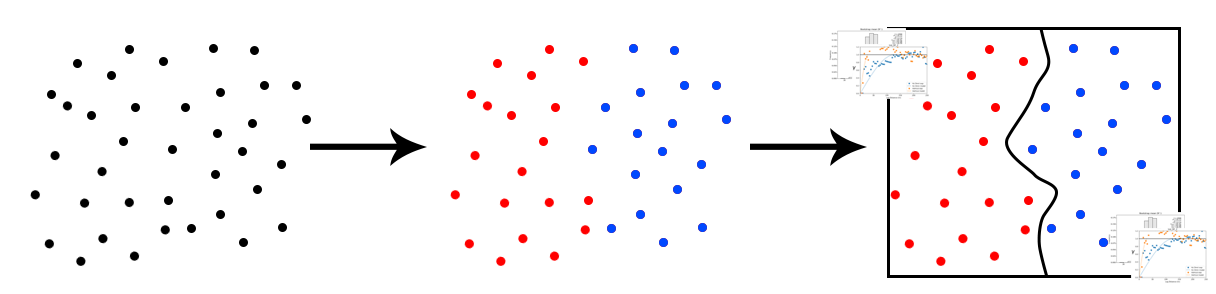
\includegraphics[width=\textwidth]{apresentacao/passo_2}
	\end{center}
\end{figure}

\end{frame}

\subsection{Método tradicional}

\begin{frame}{Metodologia tradicional}

A abordagem tradicional para a criação de modelos geológicos tridimensionais é através da triangulação de polilinhas.

\begin{figure}[H]
	\begin{center}
		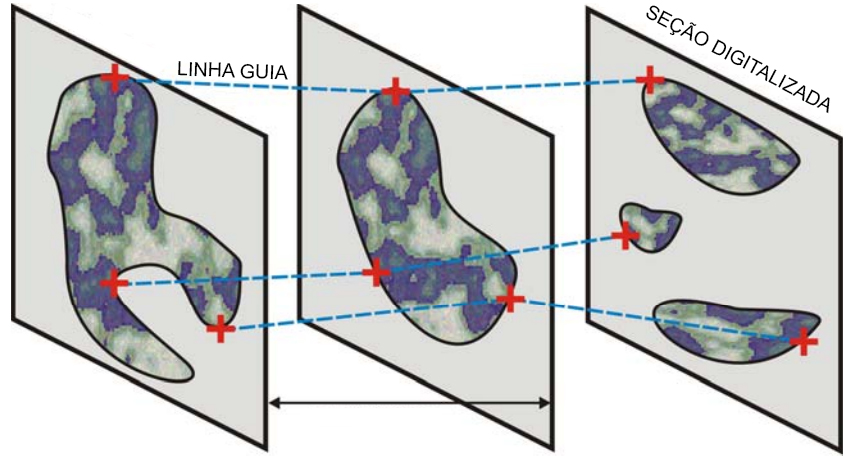
\includegraphics[width=0.6\textwidth]{capitulo_1/explicitmodeling}
	\end{center}
\end{figure}

\end{frame}

\end{document}